\documentclass[12pt]{article}
\setlength{\topmargin}{-.2in}
\setlength{\oddsidemargin}{-0cm}
\setlength{\evensidemargin}{-1cm}
\setlength{\textwidth}{16.3cm}
\setlength{\textheight}{22.3cm}
\usepackage{graphicx}
\graphicspath{{figures/}}
\usepackage[round]{natbib}
\title{Effects of Irregular Topology in Non-Planar SOM Variants}
\author{\sc{Charles R. Schmidt}\\Regional Analysis Laboratory\\Department of Geography\\San Diego State University}
%\author{\sc{Charles R. Schmidt}\\REGAL}
%\date{January 29th, 2007}
\begin{document}
\maketitle
\begin{abstract}
The development of the spherical SOM has been driven by the border effects
observed in traditional SOM.  Two problems exist with the Spherical SOM. The
first is the level of control over the network size. The second is the
topologically induced errors caused by the arrangement of neurons on the sphere.
Both of these problems stem from the problem of uniformly distributing points on
a sphere. These problems will be investigated through the introduction of a new method for
testing topologically induced errors. The method first analyzes  the neural
network to find topological mis-matches, next we train the network with an
overwhelming about of synthetic data.  Through a series of simple plots we can
then compare each neurons internal variance as defined by the variance of the
observations that best fit that neuron with suchs metrics as neighborhood
influence, number of child observations, etc.
\end{abstract}


%\section{Problem Statement}
%1. Introduction (10\%)
%\\2. Background and Lit Review (30\%)
%\\	\ldots Problem Statement
%\\	\ldots Lit Review
%\\3. Research Design / Plan / Metodology (50\%)
%\\4. Significance and Limitations (10\%)
%\\5. Timetable

\section{Introduction}
Using a Spherical lattice is widely suggested as a solution to the boundary
effect in the traditional Self-Organizing Maps \citep{ritter99, boudjemai2003,
sangole03, Wu:2006lr, Nishio:2006fk}.  However, the use of the spherical lattice
introduces a new problem.  Save the five platonic solids, distributing points on
a sphere will allows result in irregular topology \citep{ritter99}.  The classic
method for generating a spherical lattice is to tessellate the sides a platonic
solid.  When tessellating the icosahedron, as described by \cite{Wu:2006lr}, the
resulting topology will always consist of 12 pentagons and \(N-12\) hexagons.
Where \(N\) is the total number of sides, or neurons.  The main drawback of this
method is the finite control over \(N\), which grows at a rate of \(f^2*10+2\),
where \(f\) is the frequency of the tessellation \citep{Wu:2006lr}.  The goal of
this research is to investigate the effects of irregular topology within
spherical SOM.
%Find a way to incorporate finite control over N into this sentence.  A question
%that has not yet been answered is to what degree does the irregulara topology
%effect the Spherical SOM.

\section{Background and Lit Review}
The Self-Organizing Map (SOM) is an unsupervised competitive learning process
developed by Teuvo Kohonen as a technique to analyze high dimensional data sets.
The SOM algorithum uses an artificial neural network to organize high
dimensional data onto a low dimensional lattice, or map, of neurons.  Each
neuron contains a reference vector that can be considered to model a portion of
the input space. Before training these neurons are initialized, most commonly to
random values.  During the training process a randomly selected input vector
searches the map for its best matching unit (BMU), that is the neuron to which
it is most similar. The BMU and it's neiborhood, as defined by a neighborhood
function, are than adjusted to better match that observation
\citep{Kohonen2000}.  The training process is repeated a predefined number of
times, or ideally until the map converges.  The traditional SOM is laid out on a
two dimensional plane using either a rectangular or hexagonal topology.
According to \cite{Wu:2006lr} the hexagonal structure is more uniform and
generally preferred.

An obvious drawback of locating the neural lattice in a discrete euclidean plane
is the boundary of that plane.  A neruon located on the boundry has fewer
neighbors and thus fewer chances of being updated \citep{Wu:2006lr}.  The
toroidol som was introduced by \cite{li1993} and removes this drawback.
\cite{ritter99} suggests that a spherical topology may better reflect
directional data and that the torus is topologically flat.  The torus is also
less effective for visualization than the sphere, partly do to our familiarity
with maps based on the later \citep{ito2000,Wu:2006lr}.

%In the next section I review one of the primary methods for dealing with edge
%effects addressing both its features and limitations.  Following this
%discussion I introduce some simple modifications to the Spherical SOM, which
%take advantage of slightly irregular point distributions in order to yield a
%hexagonal like topology that attempts to minimize distortion.  Next a new
%method for measuring topologically caused distortion is proposed along with a
%simple numerical example.  Finally, limitations are quickly addressed and
%expected results are briefly outlined.

%\begin{figure}
%\centering
%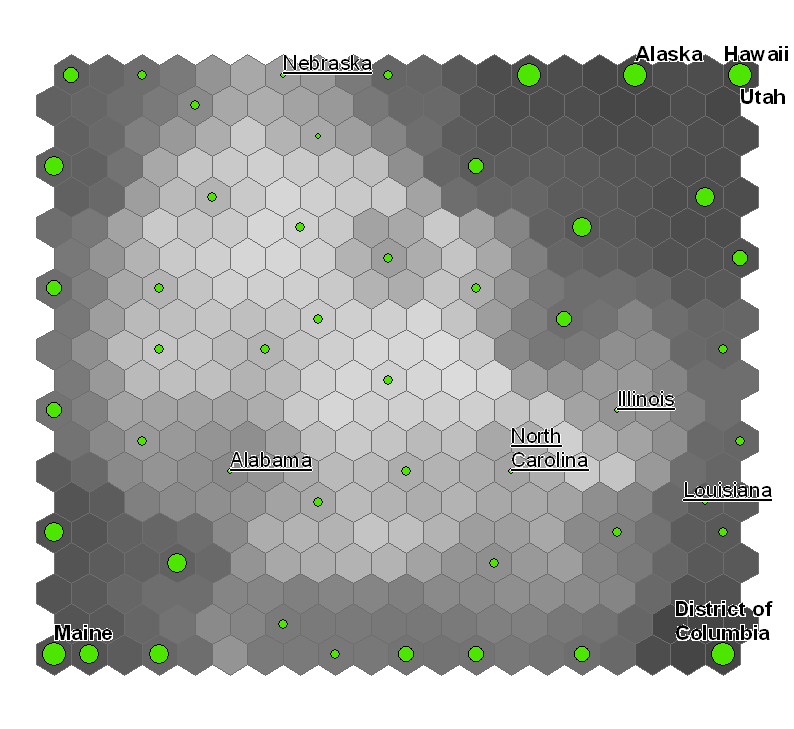
\includegraphics[width=0.85\linewidth]{gridedge.png}
%\caption{States mapped onto SOM trained with the first thirty-two census
%variables.  Darker neurons have a relatively large difference from the mean of
%the states, while lighter neurons are relatively close.}
%\label{figure1}
%\end{figure}

%\subsection{Spherical SOM}
A well-known and commonly used technique to eliminate these edge effects is to
implement the SOM algorithm on the surface of a torus or a sphere \citep{ritter99}.
\citeauthor{ritter99} first introduces the spherical SOM in
\citeyear{ritter99}, not only as a solution to the border effect, but also
suggests that a spherical SOM may better represent directional data. Several
enhancements have been suggested over \citeauthor{ritter99}'s original work
\citep{Wu:2006lr,sangole03,Nishio:2006fk,boudjemai2003}.  A good
comparison of these enhancements can be found in \citep{Wu:2006lr}.  All of
these methods derive their spherical structure through tessellations of a
polyhedron as originally proposed by \citeauthor{ritter99}.  \cite{Wu:2006lr}
point out the importance of a uniform distribution on the sphere and that is
preferable for all neurons to have an equal number of neighbors and to be
equally spaced.  They find generally that the tessellation method best
satisfies this condition and specifically that the icosahedrons is the best
starting point \citep{wu2005}.

\subsection{Network Size}
The tessellation method used by the class of spherical SOM based on Ritter's
work results in a network size that is a function of the number of
tessellations and therefore grows exponentially. In practice 2D Euclidean SOMs
also offer limited control over network size, as it is undesirable to have one
dimension dramatically larger then the other.  The literature offers little
theoretical guidance on network size \citep{cho1996}.  \cite{Nishio:2006fk}
address the issue of network size by departing from the tessellation method
and suggesting the use of a partitioned helix to uniformly distribute any
number of neurons on a sphere.  A similar method was dismissed by
\cite{wu2005} for failing to satisfy the uniformity condition.
\citeauthor{Nishio:2006fk} seem to have addressed part of the condition, the
issue of having a uniform number of direct neighbors is still not addressed.

Tessellation of the icosahedron results in a network of neurons, each of which
have exactly six neighbors, save the original twelve which each have five.
This is beneficial, as the resulting maps will share many of the same
properties as maps generated using the traditional hexagonal topology in 2D
Euclidean space. The indexed data structure developed by
\citeauthor{Wu:2006lr} (GeoSOM) allows for fast identification of direct
(first order) and indirect (\textit{n\textsuperscript{th}} order) neighbors.
\cite{Nishio:2006fk} offer no such data structure nor any practical advice on
identification of neighbors; only variance in neuron spacing is addressed.

Given that no theoretical guidance is given for choosing network size the
desire for finer control over the network size, should not be overlooked. In
particular for a larger SOM the ideal network size may not be achievable via
tessellations of the icosahedron.  In an attempt address the issue of network
size while still satisfying the uniformity condition the \cite{Rakhmanov94}
algorithm for distributing points of a sphere, which was dismissed by
\cite{wu2005} is reexamined here.  It should be noted that the method proposed
in the next section is applicable to any somewhat uniform distribution of
points on a sphere including the helix method proposed by
\cite{Nishio:2006fk}.

\section{Proposed Topology}

The Rakhmanov algorithm has the ability to distribute any number of points
onto the surface of a sphere, which allows for the finest possible level of
control of network size, even greater than that of the traditional euclidean
based SOM \citep{Rakhmanov94}.  There are two problems with the \citeauthor{Rakhmanov94}
algorithm. The first is the variance in the number of direct neighbors for any
given neuron.  The second is variance in the distance between those neurons.
Using the algorithm to distribute 162 points, results in nearest neighbor
``distances that vary from 0.15779 to 0.30069'' \cite[pg 3]{wu2005}.
Furthermore 114 neurons have 6 direct neighbors, 30 have 5 and 18 have 7, as
defined by their Delaunay Triangulation.  The fourth frequency tessellation of
the icosahedron has nearest neighbor distances in the range of 0.25319 to
0.31287, 150 neurons have 6 neighbors and 12 have 5.

Irregularities in spatial distribution of neurons exhibited by the Rakhmanov
algorithm allows a given neuron's neighboring points to be easily ranked
and sorted by their distance to the neuron in question.  The ranked and sorted
neighbors can be further separated into distinct classes, or orders, such that
the first order contains exactly \begin{math}1\times6\end{math} neurons and
the \textit{n\textsuperscript{th}} order contains exactly
\begin{math}n\times6\end{math} neurons.  Furthermore, neurons will be assigned
a distance relative to the central neuron and equal to that of their order.
For example, the six closest neurons will all be assigned a distance weight of
unity, while the next twelve closest neurons will be assigned a distance
weight of two and so on and so forth.  This follows from the properties of the
standard hexagonal topology used traditionally in SOM and provides the
foundation for a spherical SOM which mimic's that behavior.  This approach
shall be referred to as HS-SOM.

\section{Validation of Topology}
The proposed HS-SOM method raises questions of topological preservation.  One
can imagine a dense set of points evenly distributed on one hemisphere and a
sparse set of points distributed on the other. Neighborhoods near the division
would be greatly distorted; in terms of training, more updates would occur in
the dense set.  Given the overall uniformity produced by the
\citeauthor{Rakhmanov94} method this phenomenon should be minimized. However a
simple test can be conducted to check for it and further validate the HS-SOM
and other methods.

Let, \begin{math}N\end{math}, be a set of neurons.  Each neuron will have an
associated one-dimensional reference vector with its sole value initialized to
zero. Each neuron will be selected, only once, as a pseudo best matching unit
(BMU).  A constant neighborhood size will be used through out the experiment,
along with constant learning rate (set to unity).  For each BMU an input
signal (its value set to a predefined constant) shall be applied over the
BMU's neighborhood, given a standard distance decay function.  In the end,
if true edgeless hexagonal topology is preserved all neurons should have the
same value. The mean squared deviation from each node's attribute vector to
the mean attribute vector may be used as a distortion measure comparable
across any SOM, both spherical and 2D of a given network size.

It is known that for a tessellated icosahedron distortions
will be observed at exactly twelve locations on the surface, around the twelve
original vertices.  For a hexagon lattice in 2D euclidean space the
distortions will be observed at the edges of the lattice.  It is hypothesized
that for HS-SOM, distortions will be less uniform in their spatial
distribution and their overall magnitude will be less then those exhibited by
either GeoSOM or SOM\_PAK.

Further the results can be visualized to show the exact location of
topologically caused errors on the lattice.  Since we know the distortions
will occur in GeoSOM, we can use these results to help form understanding and
possibly lead to an intuitive mathematical weighting scheme for GeoSOM such as
that proposed by \cite{Kohonen2000} for 2D SOM. The method allows us to
examine the suitability of the various algorithms for uniformly distributing
points on a sphere for use in HS-SOM.

For a benchmark, the experiment is carried out over two 3x3 grids, one of
hexagonal topology, the other of rectangular topology. The neighborhood
constant is set to unity; meaning only immediate (rook contiguity) neighbors
are included. The input vector's sole value shall equal two. After each
neuron was used once as a pseudo BMU (nine training cycles) the variance of
the rectangular grid was 0.4444, while the variance of the hexagonal grid was
1.5802. As shown in figures \ref{figure2} and \ref{figure3} the hexagonal lattice
experienced higher overall values.

It should be noted that neither the potential harm nor the possible benefits
of distortions have note been explored here.  It is feasible that distortions
may help the convergence process and eliminating them entirely could
unnecessarily prolong training.

\begin{figure}
\centering
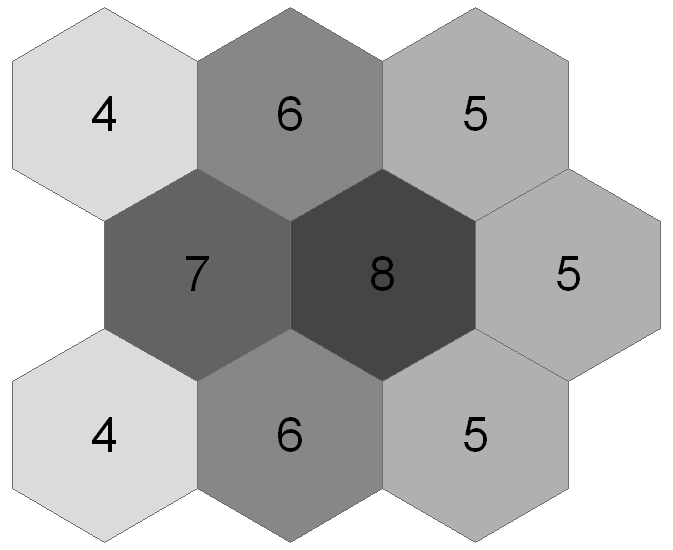
\includegraphics[width=0.4\linewidth]{figure_hex.png}
\caption{Lower numbers and lighter colors indicate topological distortion.
In the case of this specific example eight is the ideal value for all neurons
in the hexagonal lattice, two for yourself plus one for each neighbor.  For
the rectangular lattice the ideal value is six.}
\label{figure2}
\end{figure}

\begin{figure}
\centering
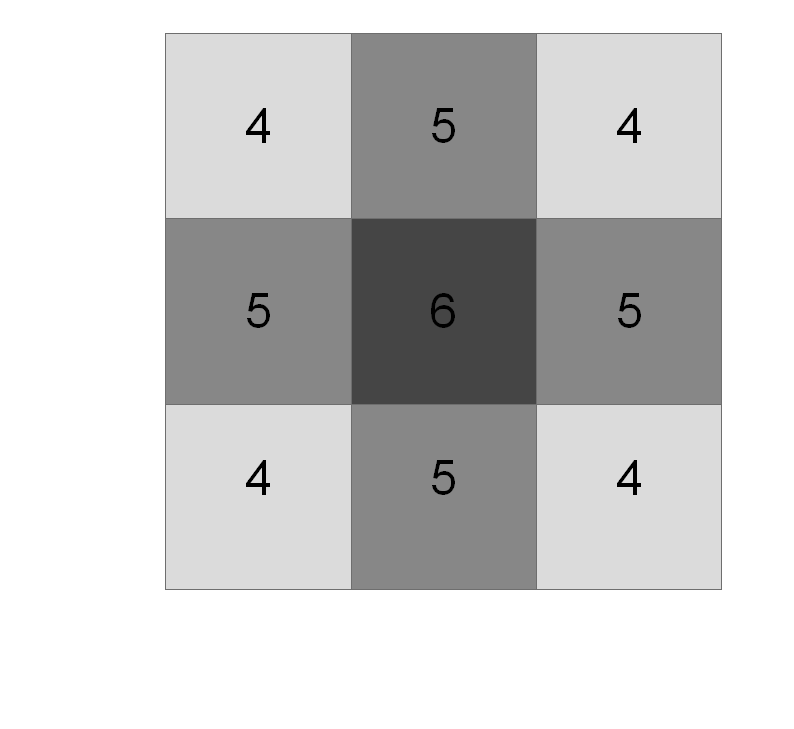
\includegraphics[width=0.4\linewidth]{figure_rect.png}
\caption{Lower numbers and lighter colors indicate topological distortion.  In
the case of this specific example eight is the ideal value for all neurons in
the hexagonal lattice, two for yourself plus one for each neighbor.  For the
rectangular lattice the ideal value is six.}
\label{figure3}
\end{figure}

\section{Limitations}
The primary limitation of the HS-SOM method is speed in neighborhood
searching. Time complexity for neighborhood searching in HS-SOM is
\begin{math}O(N)\end{math}, while GeoSOM runs in
\begin{math}O(n)\end{math}\footnote{\textit{N} is the network size and
\textit{n} in the number of neurons in the current
neighborhood}\citep{Wu:2006lr}. Time and space complexity can be reduced by
caching neighborhood calcuations on-the-fly out to the current neighborhhod
size, as opposed to precalcuting neighborhoods out to initial neighborhood
size.
\section{Expected Results and Future Work}
\begin{itemize}
\item A new tool for measuring topological preservation will be introduced.
\item HS-SOM will prove to have less distortion then 2D euclidean SOM and hopefully GeoSOM.
\item Implement the validation method and test the GeoSOM and HS-SOM using the Rakhmanov and helix methods.
\item Develop more diagnostics, such as the reverse quantization error visualizations.
\end{itemize}

%\section{Bibliography}
\bibliographystyle{apalike}
\bibliography{som}
\end{document}
